\documentclass[english, parskip=half-, 11pt]{scrartcl}

\setlength{\oddsidemargin}{0cm}
\setlength{\textwidth}{15.5cm}
\setlength{\topmargin}{-1cm}
\setlength{\textheight}{23cm}
\setlength{\parindent}{0cm}
\setlength{\parskip}{4pt}

\usepackage[utf8]{inputenc} % Inputencoding
\usepackage[T1]{fontenc} % Outputencoding
\usepackage{lmodern}
\usepackage{babel} % Umlaute, Sätze, ...
\usepackage{mathtools} % amsmath erweitert
\usepackage{amssymb} % mathematische Symbole
%\usepackage{fancyhdr} % Kopf- und Fußzeilen
\usepackage{microtype} % Randausgleich, Umbrüche, ...
\usepackage{xcolor}
\usepackage{csquotes}
%\usepackage{MnSymbol}
\usepackage[hidelinks]{hyperref}
\usepackage{enumerate}

\usepackage{tikz} % Grafiken
\usetikzlibrary{calc}
\usepackage{circuitikz}
%\usepackage{tikz-3dplot}
%\usetikzlibrary{arrows,decorations.pathmorphing}
%\usepackage{siunitx} % Einheiten
%\sisetup{locale=DE} % Konfiguration zu siunitx
%\usepackage{booktabs} % Tabellen
%\usepackage{pdfpages}
\usepackage{float}
\usepackage{listings}

\usepackage{enumitem}
%\setlist[description]{font=\normalfont}
%\setlength{\parindent}{0pt}
\renewcommand\labelitemi{--}
\newcommand{\topSection}[1]{{\bfseries {#1}}}
\newcommand{\itemizeMargin}{3cm}
\newcommand{\itemizeIndent}{-2cm}

\newcommand{\radius}{.65}

% default parameters
\newcommand{\icLabel}{\large Label}
\newcommand{\pinNamesLeft}{0/pin0, 1/pin1, 2/pin2, 3/pin3, 4/pin4, 5/pin5, 6/pin6, 7/pin7} % 0 up to \pinCountPerSide-1
\newcommand{\pinNamesRight}{8/pin8, 9/pin9, 10/pin10, 11/pin11, 12/pin12, 13/pin13, 14/pin14, 15/pin15} % \pinCountPerSide up to 2*\pinCountPerSide-1
\newcommand{\icWidth}{4}
\newcommand{\icHeight}{10}
\newcommand{\pinCountPerSide}{8}
\newcommand{\pinWidth}{1.05}
\newcommand{\pinHeight}{.49}
\newcommand{\pinDistance}{1.27}
\newcommand{\markerDiameter}{1.333333333333333333333}
\newcommand{\labelOffset}{1}
\newcommand{\globalRotation}{0}
\newcommand{\textRotation}{90}
\newcommand{\pinTextRotation}{0}
\newcommand{\labelAnchor}{west}
\newcommand{\textRightAnchor}{west}
\newcommand{\textLeftAnchor}{east}

% common
\newcommand{\invertPin}[1]{$\overline{\text{#1}}$}
\newcommand{\ground}{\text{GND}}
\newcommand{\vcc}{\text{VCC}}
\newcommand{\vccPeriphery}{\text{VCCo}}
\newcommand{\serialIn}{\text{SER}}
\newcommand{\outputEnable}{\text{OE}}
\newcommand{\notConnected}{\text{NC}}
\newcommand{\signalHigh}{HIGH}
\newcommand{\signalLow}{LOW}
\newcommand{\mosi}{MOSI}
\newcommand{\miso}{MISO}
\newcommand{\reset}{Reset}
\newcommand{\clock}{CLK}
\newcommand{\spi}{SPI}

% ATmega328P specific
\newcommand{\atmegathreetwoeightp}{ATmega328P}
\newcommand{\avcc}{AVCC}
\newcommand{\aref}{AREF}
\newcommand{\xtal}{XTAL}

% shift-register specific
\newcommand{\shiftRegisterName}{\text{74HC595}}
\newcommand{\shiftRegisterClockOut}{RCLK}
\newcommand{\shiftRegisterClockIn}{SRCLK}
\newcommand{\shiftRegisterClear}{SRCLR}
\newcommand{\shiftRegisterInternalBit}{\text{q}}
\newcommand{\shiftRegisterExternalBit}{\text{Q}}
\newcommand{\shiftRegisterSerialOut}{$\shiftRegisterInternalBit_{7}$}
\newcommand{\shiftRegisterSerialIn}{\serialIn}
\newcommand{\shiftRegisterOutputEnable}{\OutputEnable} % Todo: check nested commands!

% parallel-load specific
\newcommand{\parallelLoadName}{\text{74HC165}}
\newcommand{\parallelLoadParallelLoad}{PL}
\newcommand{\parallelLoadClock}{CP}
\newcommand{\parallelLoadClockEnable}{CE}
\newcommand{\parallelLoadSerialIn}{\serialIn}
\newcommand{\parallelLoadInternalBit}{\text{d}}
\newcommand{\parallelLoadExternalBit}{\text{D}}
\newcommand{\parallelLoadSerialOut}{$\parallelLoadInternalBit_{7}$}

% r/s-latch specific
\newcommand{\latchName}{\text{CD4043B}}
\newcommand{\latchReset}{\text{R}}
\newcommand{\latchSet}{\text{S}}
\newcommand{\latchOutput}{\text{Q}}
\newcommand{\latchOutputEnable}{\outputEnable}
\newcommand{\latchNotConnected}{\notConnected}

% outputs
\newcommand{\additionalPinsOneName}{\text{connectorLeft}}
\newcommand{\additionalPinsTwoName}{\text{connectorRight}}
\newcommand{\pinOut}{\text{Out}}
\newcommand{\pinIn}{\text{In}}

\newcommand{\devicePinConcatenation}[2]{{#1} - {#2}}


\title{Button Matrix - Documentation}
\author{Johannes Wilde}

\begin{document}

\begin{center}
	\Huge \underline{Button Matrix - Documentation}\\
	{\normalsize \textbf{Revision 1}}
\end{center}

\vspace*{-1cm}

\section{Circuit Board}

\subsection{Schematic}

\begin{figure}[H]
	\centering
	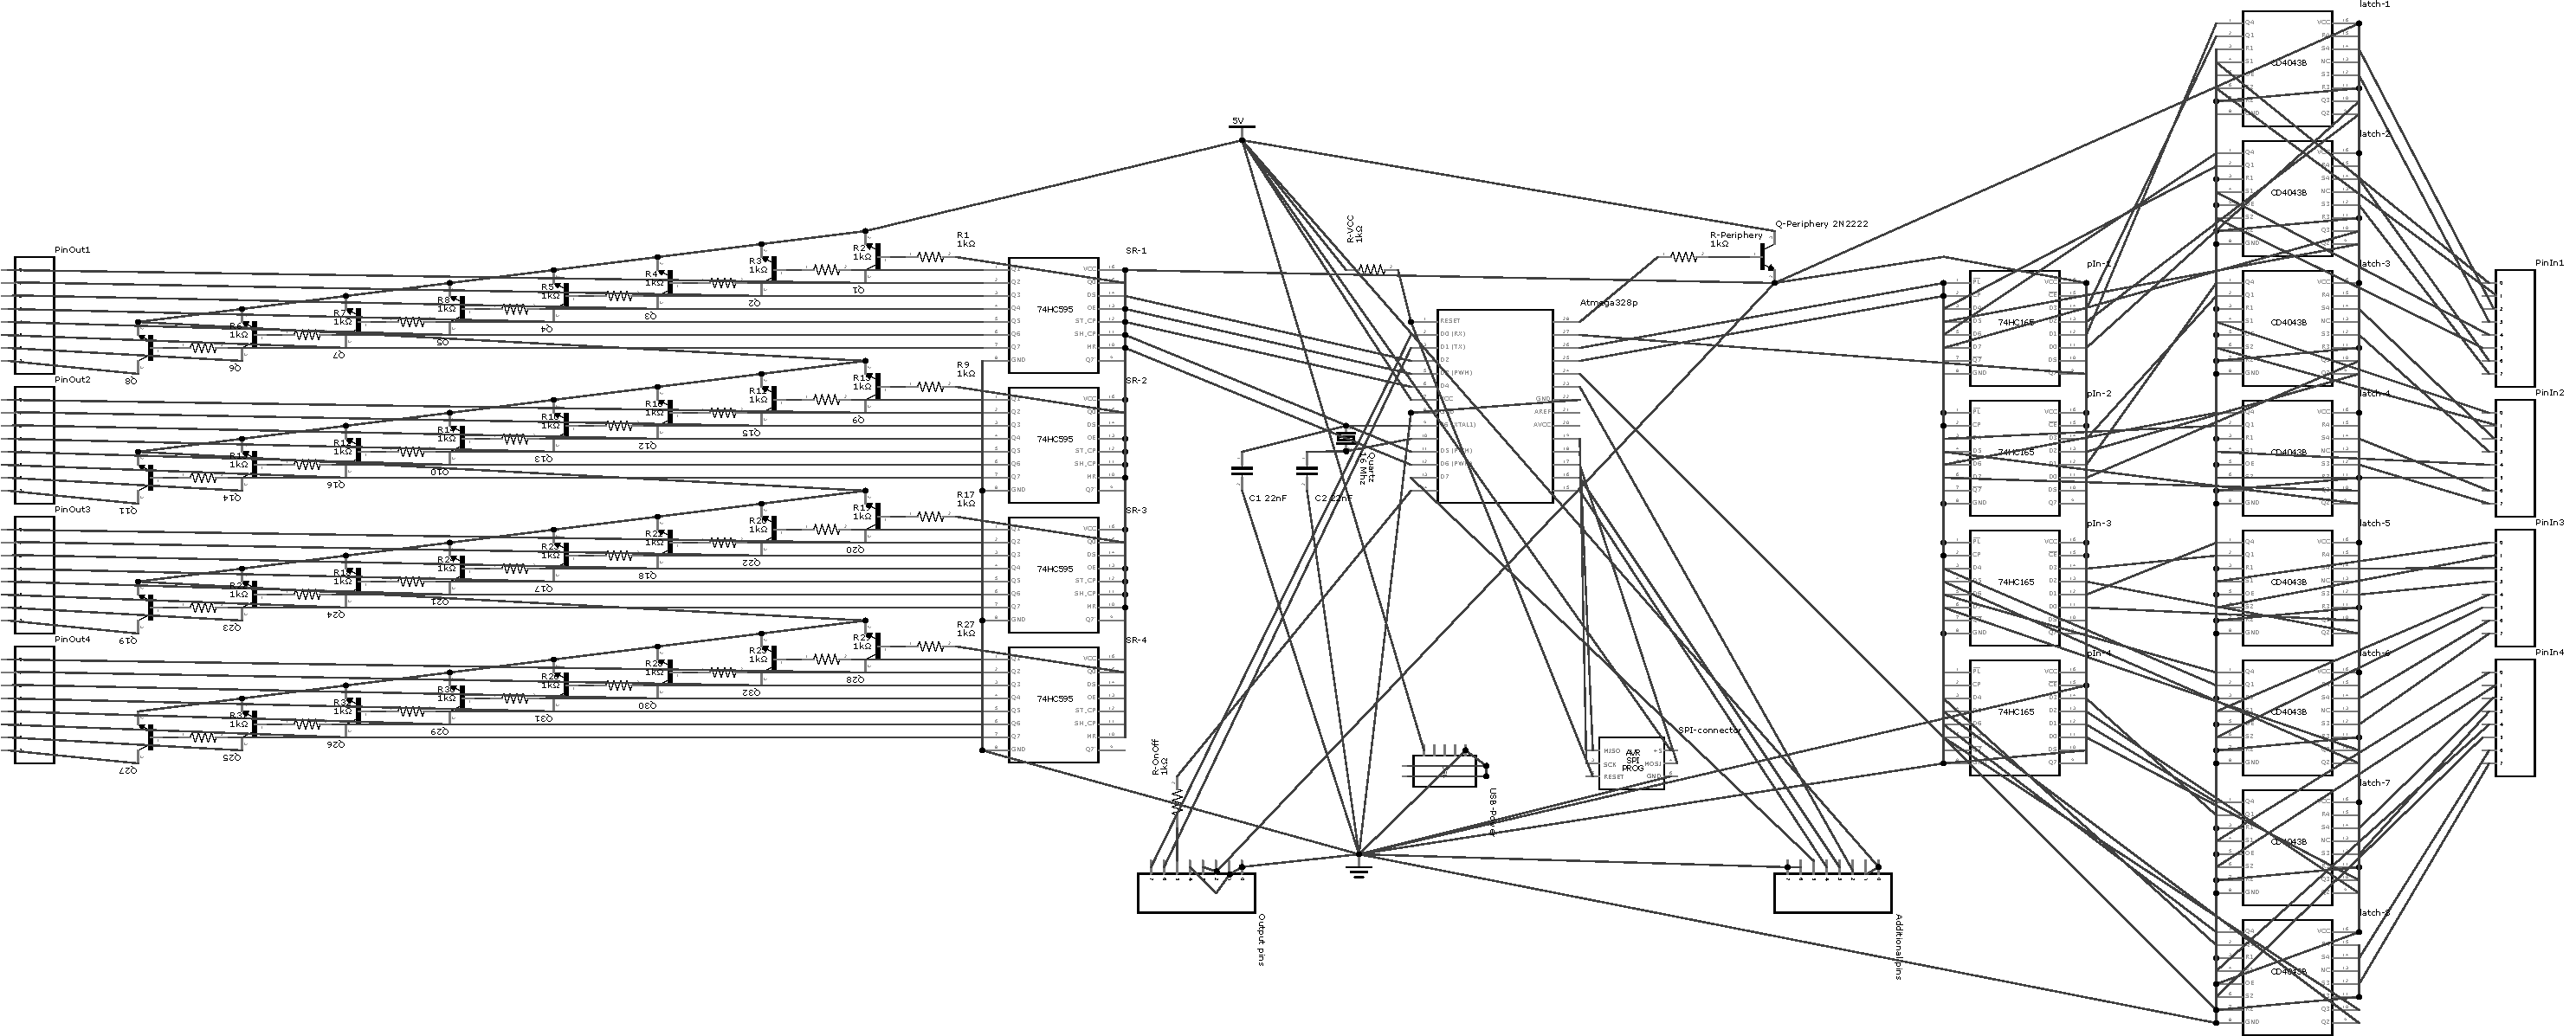
\includegraphics[width=\textwidth]{./Images/201902_GameBoard_schem-v1.pdf}
	\caption{Schematic view of the circuit board design.}
	\label{fig:schematic}
\end{figure}
%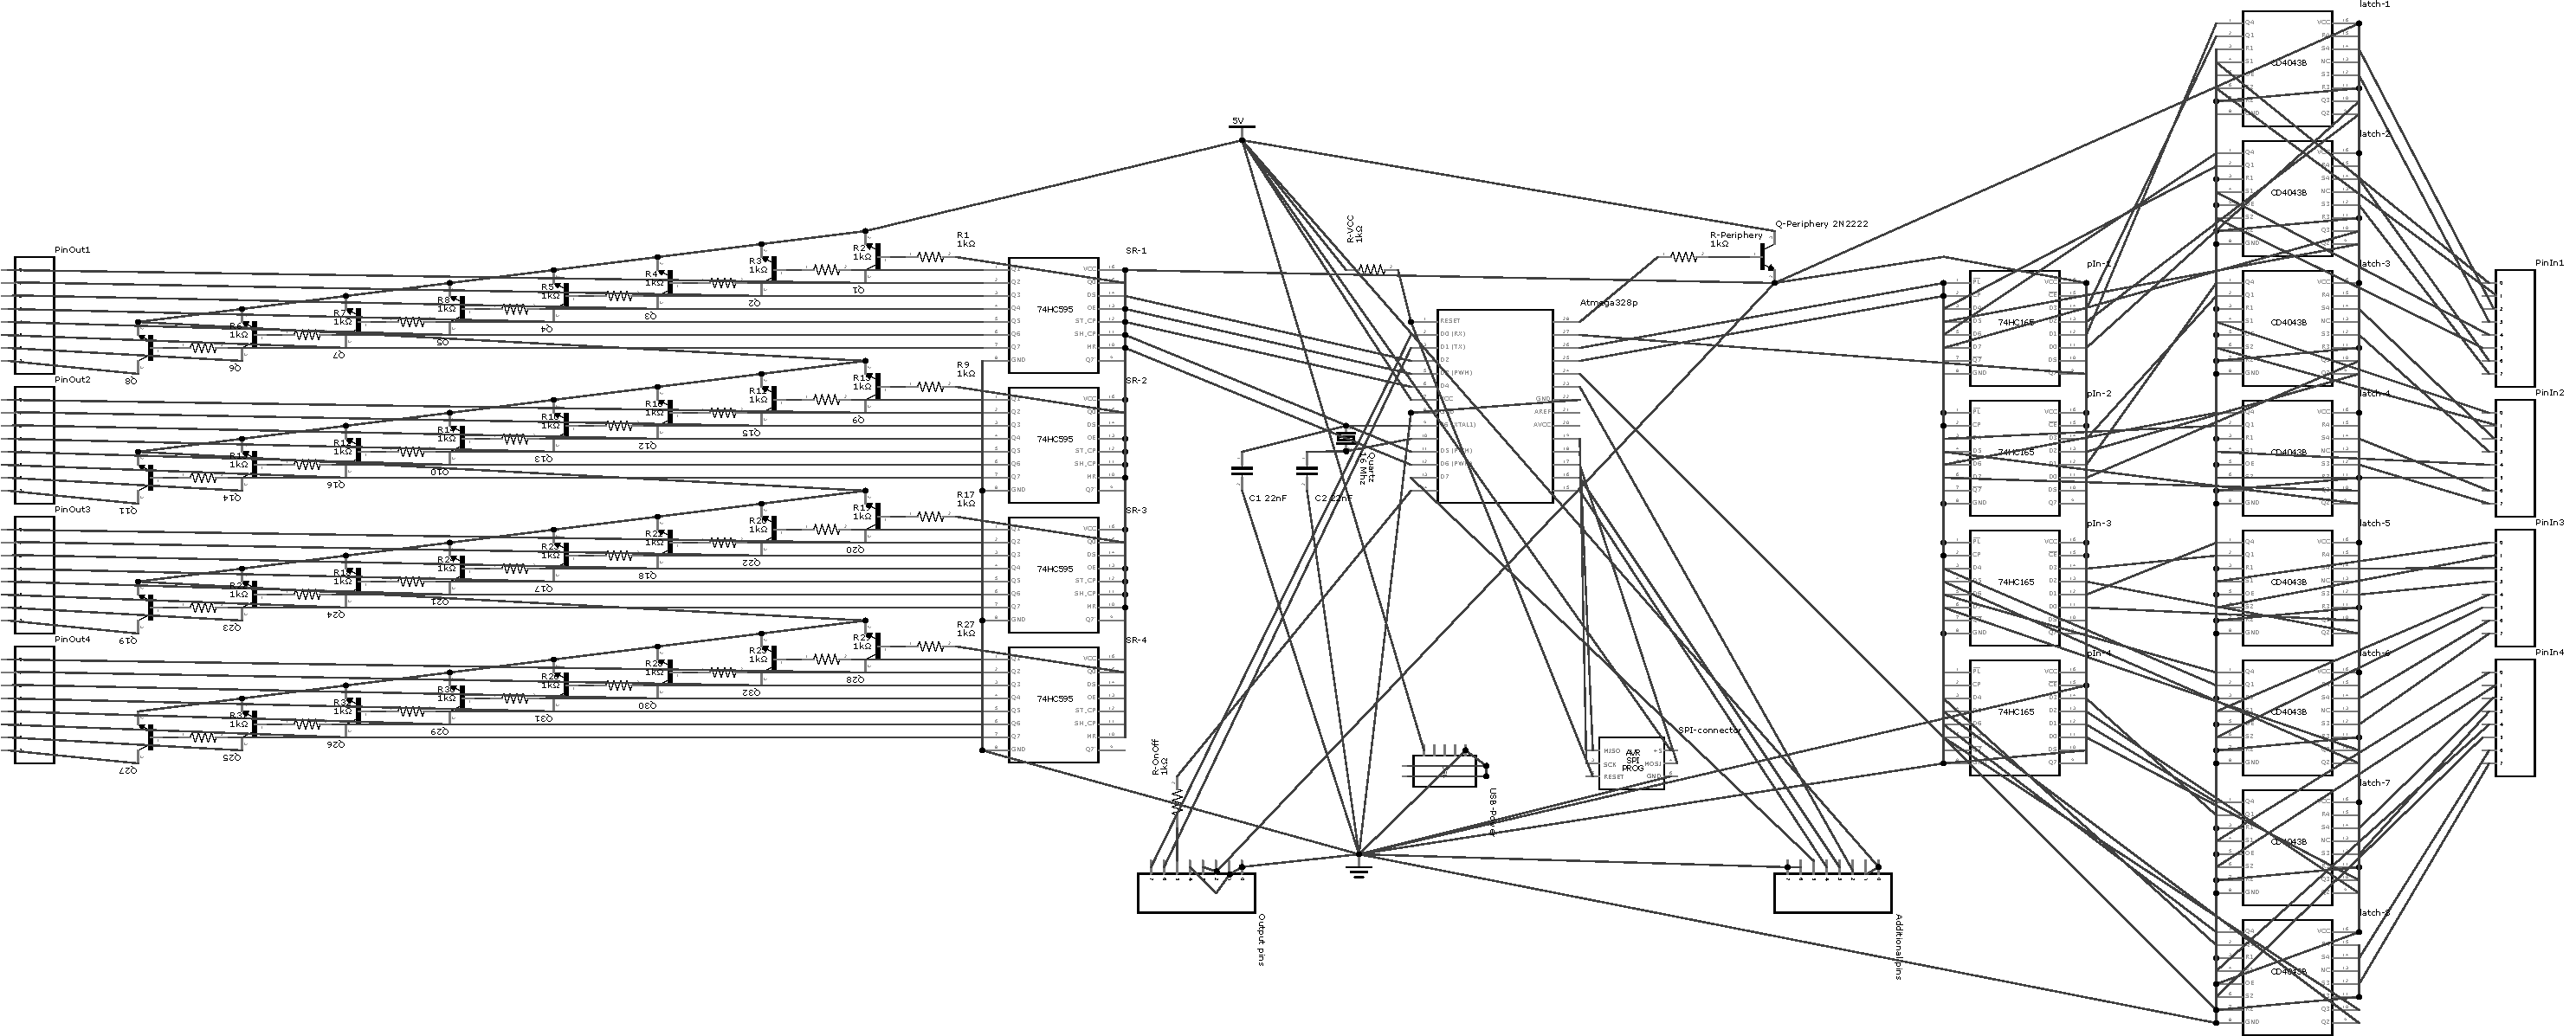
\includepdf[fitpaper=true, pages=-]{./Images/201902_GameBoard_schem-v1.pdf}


\subsection{Layout - Top}

\begin{figure}[H]
	\centering
	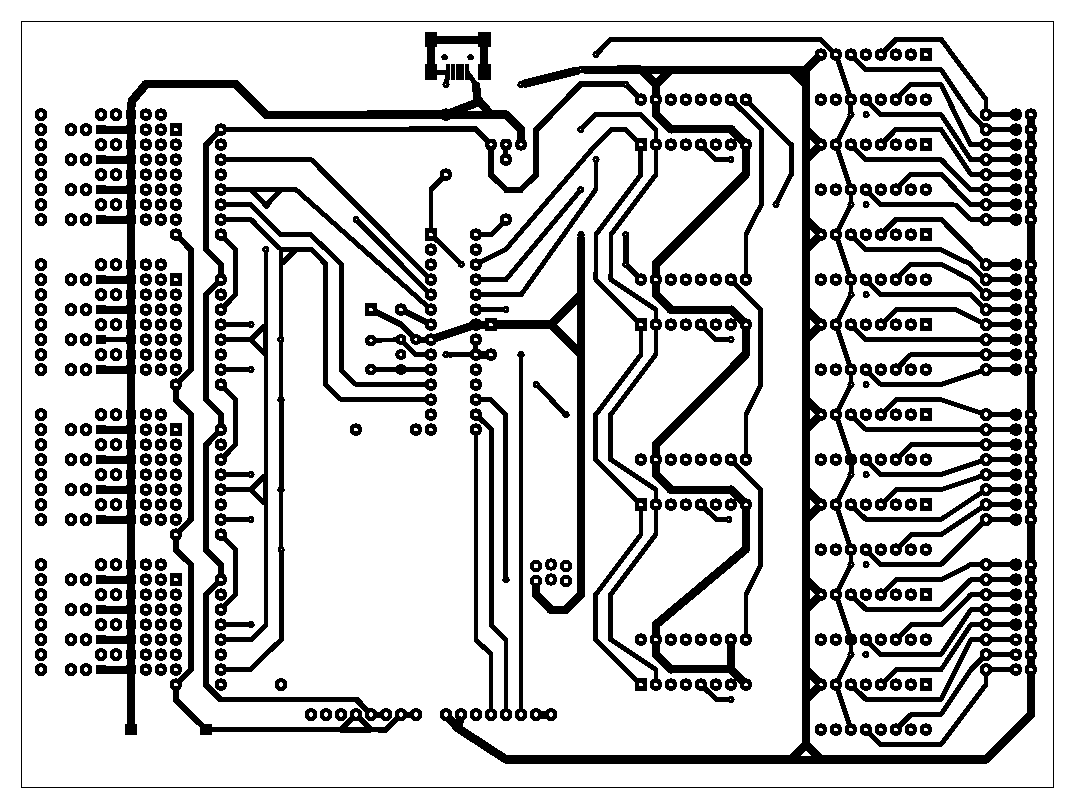
\includegraphics[width=.7\textwidth]{./Images/201902_GameBoard_fudged_final1_etch_copper_top.pdf}
	\caption{View of the circuit board top as seen from the top.}
	\label{fig:circuitTop}
\end{figure}

\subsection{Layout - Bottom}

\begin{figure}[H]
	\centering
	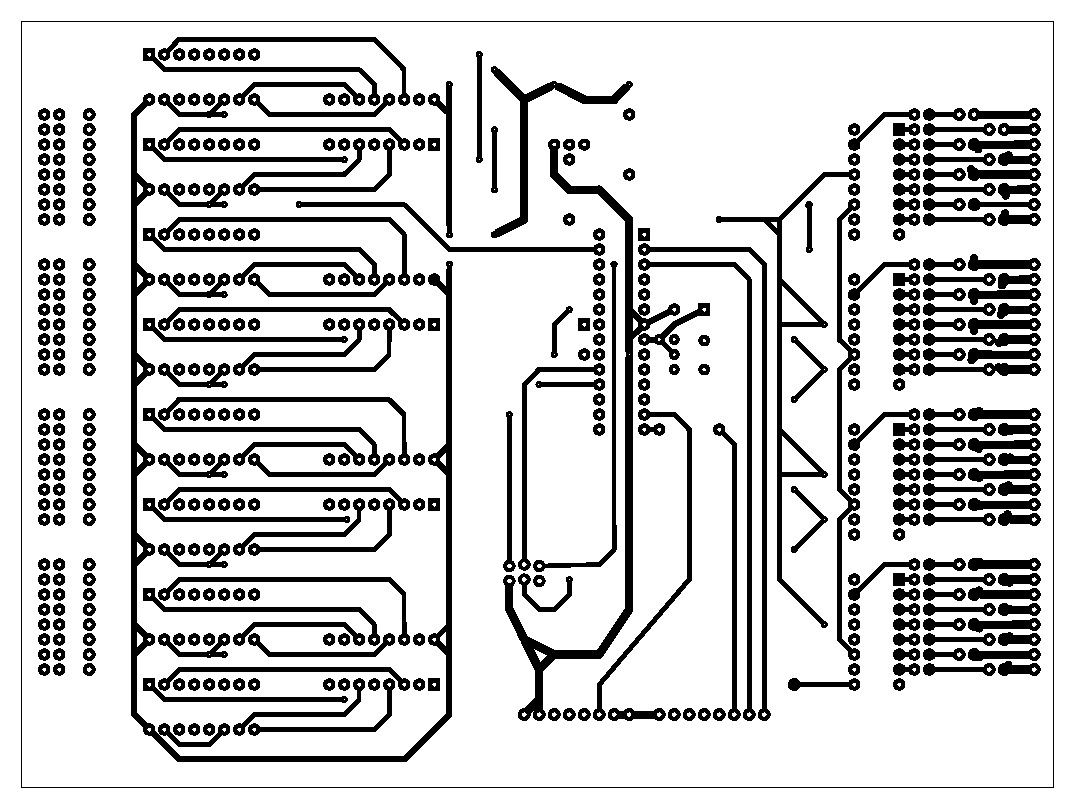
\includegraphics[width=.7\textwidth]{./Images/201902_GameBoard_fudged_final1_etch_copper_bottom_mirror.pdf}
	\caption{View of the circuit board bottom as seen from the bottom.}
	\label{fig:circuitBottom}
\end{figure}

\subsection{Layout - Hardware}

\begin{figure}[H]
	\centering
	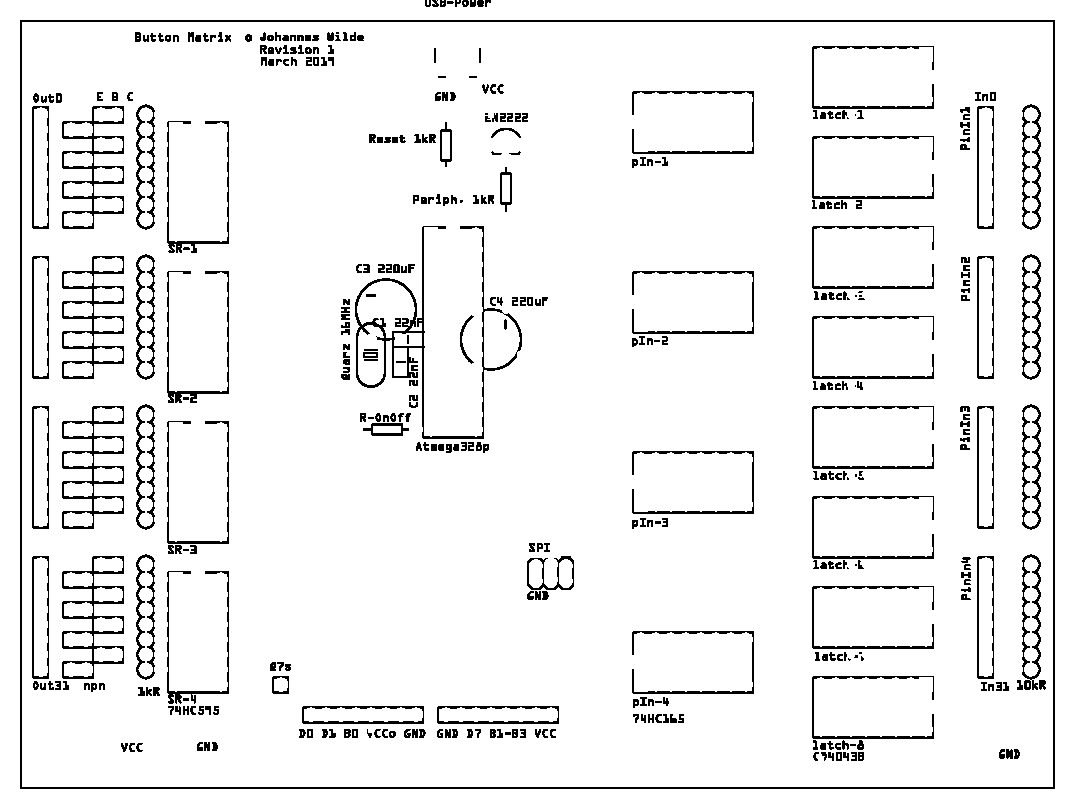
\includegraphics[width=.7\textwidth]{./Images/201902_GameBoard_fudged_final1_grounded_named_etch_silk_top.pdf}
	\caption{Positioning of the hardware as seen from the top.}
	\label{fig:hardwareTop}
\end{figure}


\subsection{Pin Connections}


\begin{table}[H]
	\centering
	\caption{Pins of the \atmegathreetwoeightp\ and their respective connections.}
	\label{tab:atmega328pConnections}
	\begin{tabular}{c|l}
		\atmegathreetwoeightp\ pin  & connected to \\\hline
		\vcc & \vcc\\
		\ground & \ground\\
		\aref & \vcc\\
		\avcc & \vcc\\
		B0 & \devicePinConcatenation{\additionalPinsOneName}{5}\\
		B1 & \devicePinConcatenation{\additionalPinsTwoName}{4}\\
		B2 & \devicePinConcatenation{\additionalPinsTwoName}{3}\\
		B3 & \devicePinConcatenation{\spi}{\mosi}\\
		B4 & \devicePinConcatenation{\spi}{\miso}\\
		B5 & \devicePinConcatenation{\spi}{\clock}\\
		B6 & \xtal\\
		B7 & \xtal\\
		C0 & \devicePinConcatenation{\additionalPinsTwoName}{2}\\
		C1 & \devicePinConcatenation{\latchName}{$\latchReset_i$}\\
		C2 & \devicePinConcatenation{\parallelLoadName}{\parallelLoadClock}\\
		C3 & \devicePinConcatenation{\parallelLoadName}{\invertPin{\parallelLoadParallelLoad}}\\
		C4 & \devicePinConcatenation{\parallelLoadName}{$\parallelLoadInternalBit_{7}$}\\
		C5 & \vccPeriphery\ enable\\
		C6 & \invertPin{\reset}\\
		D0 & \devicePinConcatenation{\additionalPinsOneName}{7}\\
		D1 & \devicePinConcatenation{\additionalPinsOneName}{6}\\
		D2 & \devicePinConcatenation{\shiftRegisterName}{\serialIn}\\
		D3 & \devicePinConcatenation{\shiftRegisterName}{\invertPin{\outputEnable}}\\
		D4 & \devicePinConcatenation{\shiftRegisterName}{\shiftRegisterClockOut}\\
		D5 & \devicePinConcatenation{\shiftRegisterName}{\shiftRegisterClockIn}\\
		D6 & \devicePinConcatenation{\shiftRegisterName}{\invertPin{\shiftRegisterClear}}\\
		D7 & \devicePinConcatenation{\additionalPinsTwoName}{5}\\
	\end{tabular}
\end{table}

\begin{table}[H]
	\centering
	\caption{Pins of the \shiftRegisterName\ and their respective connections.}
	\label{tab:shiftregisterConnections}
	\begin{tabular}{c|l}
		\shiftRegisterName\ pin  & connected to \\\hline
		\vcc & \vccPeriphery\\
		\ground & \ground\\
		\serialIn & \devicePinConcatenation{\atmegathreetwoeightp}{D2} / \devicePinConcatenation{$\shiftRegisterName^{\prime\prime}$}{\shiftRegisterSerialOut}\\
		\invertPin{\outputEnable} & \devicePinConcatenation{\atmegathreetwoeightp}{D3}\\
		\shiftRegisterClockOut & \devicePinConcatenation{\atmegathreetwoeightp}{D4}\\
		\shiftRegisterClockIn & \devicePinConcatenation{\atmegathreetwoeightp}{D5}\\
		\invertPin{\shiftRegisterClear} & \devicePinConcatenation{\atmegathreetwoeightp}{D6}\\
		$\shiftRegisterInternalBit_{7}$ & \devicePinConcatenation{$\shiftRegisterName^{\prime}$}{\serialIn} / \notConnected\\
		$\shiftRegisterExternalBit_{i}$ & $\pinOut_j$-transistor base
	\end{tabular}
\end{table}

\begin{table}[H]
	\centering
	\caption{Pins of the \parallelLoadName\ and their respective connections.}
	\label{tab:parallelLoadConnections}
	\begin{tabular}{c|l}
		\parallelLoadName\ pin  & connected to \\\hline
		\vcc & \vccPeriphery\\
		\ground & \ground\\
		\invertPin{\parallelLoadParallelLoad} & \devicePinConcatenation{\atmegathreetwoeightp}{C3}\\
		\parallelLoadClock & \devicePinConcatenation{\atmegathreetwoeightp}{C2}\\
		\parallelLoadSerialOut & \devicePinConcatenation{\atmegathreetwoeightp}{C4} / \devicePinConcatenation{$\parallelLoadName^{\prime\prime}$}{\parallelLoadSerialIn}\\
		\invertPin{\parallelLoadSerialOut} & \notConnected\\
		\parallelLoadSerialIn & \devicePinConcatenation{$\parallelLoadName^{\prime}$}{\parallelLoadSerialOut} / \ground\\
		\invertPin{\parallelLoadClockEnable} & \ground\\
		$\parallelLoadExternalBit_i$ & \devicePinConcatenation{\latchName}{$\latchOutput_i$}\\
	\end{tabular}
\end{table}

\begin{table}[H]
	\centering
	\caption{Pins of the \latchName\ and their respective connections.}
	\label{tab:latchConnections}
	\begin{tabular}{c|l}
		\latchName\ pin  & connected to \\\hline
		\vcc & \vccPeriphery\\
		\ground & \ground\\
		$\latchOutput_i$ & \devicePinConcatenation{\parallelLoadName}{$\parallelLoadExternalBit_j$}\\
		$\latchSet_i$ & $\pinIn_{k}$\\
		$\latchReset_i$ & \devicePinConcatenation{\atmegathreetwoeightp}{C1}\\
		\latchOutputEnable & \vccPeriphery\\
	\end{tabular}
\end{table}

\begin{table}[H]
	\centering
	\caption{Pins of the \additionalPinsOneName\ and their respective connections.}
	\label{tab:additionalPinsOneConnections}
	\begin{tabular}{c|l}
		\additionalPinsOneName\ pin  & connected to \\\hline
		0 & \ground\\
		1 & \ground\\
		2 & \vccPeriphery\\
		3 & \vccPeriphery\\
		4 & \ground\\
		5 & \atmegathreetwoeightp-B0\\
		6 & \atmegathreetwoeightp-D1\\
		7 & \atmegathreetwoeightp-D0\\
	\end{tabular}
\end{table}

\begin{table}[H]
	\centering
	\caption{Pins of the \additionalPinsTwoName\ and their respective connections.}
	\label{tab:additionalPinsTwoConnections}
	\begin{tabular}{c|l}
		\additionalPinsTwoName\ pin  & connected to \\\hline
		0 & \vcc\\
		1 & \vcc\\
		2 & \atmegathreetwoeightp-C0\\
		3 & \atmegathreetwoeightp-B2\\
		4 & \atmegathreetwoeightp-B1\\
		5 & \atmegathreetwoeightp-D7\\
		6 & \ground\\
		7 & \ground\\
	\end{tabular}
\end{table}

Above notations are held rather general - for the actual connections please refer to the schematic or board layouts above.

For better understandability however some general remarks:
\begin{enumerate}
	\item The devices containing shiftregisters [\shiftRegisterName, \parallelLoadName] are concatenated with those of the same type, i.e.\ one device's output is connected to the next device's input [e.g.\ for \shiftRegisterName\ it is \shiftRegisterSerialOut\ of the next one connected to \shiftRegisterSerialIn\ of the previous one]. This is supposed to be inferred when using $\empty^{\prime}$ in above tables.
	\item The last device in those concatenations is somewhat special, insofar as that for \shiftRegisterName\ \shiftRegisterSerialOut\ is \notConnected\ and for \parallelLoadName\ \parallelLoadSerialIn\ is connected to \ground.\\
	And for the first device \shiftRegisterName\ \shiftRegisterSerialIn\ is connected to \devicePinConcatenation{\atmegathreetwoeightp}{D2}\ and for \parallelLoadName\ \parallelLoadSerialOut\ is connected to \devicePinConcatenation{\atmegathreetwoeightp}{C4}.
	\item The connection of the \shiftRegisterName\ to the \pinOut\ is rather straightforward: the first output of the first shiftregister in the concatenation is connected to the first \pinOut\ and the last output of the last shiftregister in the concatenation is connected to the last \pinOut.
	\item For \pinIn\ this is somewhat more complicated:\\
\begin{center}
	\begin{tabular}{c|c}
		\parallelLoadName\ pin & \pinIn\ pin \\\hline
		0 & 3\\
		1 & 2\\
		2 & 1\\
		3 & 0\\
		4 & 4\\
		5 & 5\\
		6 & 6\\
		7 & 7
	\end{tabular}
\end{center}
	
\end{enumerate}


\pagebreak

\section{Hardware Description}

\subsection{\atmegathreetwoeightp}

\begin{figure}[h!]
	\centering
	\begin{tikzpicture}[scale=.37]
		\renewcommand{\icWidth}{4}
		\renewcommand{\icHeight}{18}
		\renewcommand{\pinCountPerSide}{14}
		
		\renewcommand{\icLabel}{\large \atmegathreetwoeightp}
		
		\renewcommand{\pinNamesLeft}{0/{(\invertPin{\reset}) C6}, 1/{(RX) D0}, 2/{(TX) D1}, 3/D2, 4/D3, 5/D4, 6/\vcc, 7/\ground, 8/{(\xtal1) B6}, 9/{(\xtal2) B7}, 10/D5, 11/D6, 12/D7, 13/B0} % 0 up to \pinCountPerSide-1
		\renewcommand{\pinNamesRight}{14/B1, 15/B2, 16/{B3 (\mosi)}, 17/{B4 (\miso)}, 18/{B5 (\clock)}, 19/\avcc, 20/\aref, 21/\ground, 22/C0, 23/C1, 24/C2, 25/C3, 26/C4, 27/C5} % \pinCountPerSide up to 2*\pinCountPerSide-1
		
		\begin{scope}[xshift=23cm,yshift=-12cm, rotate=\globalRotation]
			\foreach \pinNumber/\name in \pinNamesLeft
			{
				\draw (0,\icHeight - \icHeight / 2 + \pinCountPerSide * \pinDistance / 2 - 1 * \pinDistance / 2 - \pinNumber * \pinDistance - \pinHeight / 2) rectangle ++(-\pinWidth,\pinHeight) ++(0,-\pinHeight/2) node[anchor=\textLeftAnchor, rotate=\pinTextRotation] {\name};
			}
			\pgfmathparse{\pinCountPerSide - 1}
			\foreach \pinNumber/\name in \pinNamesRight
			{
				\draw (\icWidth,-\icHeight / 2 - \pinCountPerSide * \pinDistance / 2 + 1 * \pinDistance / 2 + \pinNumber * \pinDistance - \pinHeight / 2) rectangle ++(\pinWidth,\pinHeight) ++(0,-\pinHeight/2) node[anchor=\textRightAnchor, rotate=\pinTextRotation] {\name};
			}
			\draw[thick] (0,0) -- ++(\icWidth,0) -- ++(0,\icHeight) -- ++(-1*\icWidth/2+\markerDiameter/2,0) arc (0:-180:\markerDiameter/2) -- ++(-1*\icWidth/2+\markerDiameter/2,0) -- ++(0,-\icHeight);
			
			\draw (\icWidth/2,\labelOffset) node[anchor=\labelAnchor, rotate=\textRotation] {\icLabel};
		\end{scope}
	\end{tikzpicture}
	\caption{Schematic of the \atmegathreetwoeightp.}
	\label{fig:atmega328p}
\end{figure}

The bracketed names specify functionality assigned to the respective pins by the underlying hardware design. If one would want, these can be reconfigured for different use cases however.


\subsection{\shiftRegisterName\ - 8-bit Shift Register}

\begin{figure}[h!]
	\centering
	\begin{tikzpicture}[scale=.37]
	
		\renewcommand{\icLabel}{\large \shiftRegisterName}
		
		\renewcommand{\pinNamesLeft}{0/$\shiftRegisterExternalBit_1$, 1/$\shiftRegisterExternalBit_2$, 2/$\shiftRegisterExternalBit_3$, 3/$\shiftRegisterExternalBit_4$, 4/$\shiftRegisterExternalBit_5$, 5/$\shiftRegisterExternalBit_6$, 6/$\shiftRegisterExternalBit_7$, 7/\ground} % 0 up to \pinCountPerSide-1
		\renewcommand{\pinNamesRight}{8/\shiftRegisterSerialOut, 9/\invertPin{\shiftRegisterClear}, 10/\shiftRegisterClockIn, 11/\shiftRegisterClockOut, 12/\invertPin{\outputEnable}, 13/\shiftRegisterSerialIn, 14/$\shiftRegisterExternalBit_0$, 15/\vcc} % \pinCountPerSide up to 2*\pinCountPerSide-1
			
		\begin{scope}[xshift=23cm,yshift=-12cm, rotate=\globalRotation]
			\foreach \pinNumber/\name in \pinNamesLeft
			{
				\draw (0,\icHeight - \icHeight / 2 + \pinCountPerSide * \pinDistance / 2 - 1 * \pinDistance / 2 - \pinNumber * \pinDistance - \pinHeight / 2) rectangle ++(-\pinWidth,\pinHeight) ++(0,-\pinHeight/2) node[anchor=\textLeftAnchor, rotate=\pinTextRotation] {\name};
			}
			\pgfmathparse{\pinCountPerSide - 1}
			\foreach \pinNumber/\name in \pinNamesRight
			{
				\draw (\icWidth,-\icHeight / 2 - \pinCountPerSide * \pinDistance / 2 + 1 * \pinDistance / 2 + \pinNumber * \pinDistance - \pinHeight / 2) rectangle ++(\pinWidth,\pinHeight) ++(0,-\pinHeight/2) node[anchor=\textRightAnchor, rotate=\pinTextRotation] {\name};
			}
			\draw[thick] (0,0) -- ++(\icWidth,0) -- ++(0,\icHeight) -- ++(-1*\icWidth/2+\markerDiameter/2,0) arc (0:-180:\markerDiameter/2) -- ++(-1*\icWidth/2+\markerDiameter/2,0) -- ++(0,-\icHeight);
			
			\draw (\icWidth/2,\labelOffset) node[anchor=\labelAnchor, rotate=\textRotation] {\icLabel};
		\end{scope}
	\end{tikzpicture}
    \caption{Schematic of the 8-bit shift register \shiftRegisterName.}
    \label{fig:shiftRegister}
\end{figure}
Working principle:\\
The shiftregister has an internal [$\shiftRegisterInternalBit_i$, $i \in [0,7]$] and an external [$\shiftRegisterExternalBit_i$, $i \in [0,7]$] 8-bit register.\\
On a rising edge on \shiftRegisterClockIn\ the values $\shiftRegisterInternalBit_i$ are shifted to $\shiftRegisterInternalBit_{i+1}$ [$i \in [0,6]$, higher $i$ first] and \shiftRegisterSerialIn\ to $\shiftRegisterInternalBit_0$.\\
On a rising edge on \shiftRegisterClockOut\ the values of $\shiftRegisterInternalBit_i$ are copied to $\shiftRegisterExternalBit_{i}$ [$i \in [0,7]$]. These will only be visible externally if \invertPin{\outputEnable}\ is \signalLow\ [otherwise the outputs will be in a high impedance state].\\
A \signalLow\ on \invertPin{\shiftRegisterClear}\ will set $\shiftRegisterInternalBit_i$ [$i \in [0,7]$] \signalLow.\\
\vcc\ and \ground\ are required for the shift-register to work.\\
\shiftRegisterSerialOut\ can be used to pass the out-shifted bits on to another shift-register, if \shiftRegisterSerialOut\ is connected to \shiftRegisterSerialIn\ of the next shift-register [which will have to be clocked accordingly].

$\shiftRegisterExternalBit_i$ - Output $i$; \ground\ - Ground; \shiftRegisterSerialOut\ - Serial output; \invertPin{\shiftRegisterClear} - Clear internal shift-register on \signalLow; \shiftRegisterClockOut\ - Copy internal to external shift-register; \shiftRegisterClockIn\ - shift in \serialIn\ on rising edge; \invertPin{\outputEnable} - Output Enable; \serialIn\ - Serial input; \vcc\ - Supply Voltage.
%\newpage

\subsection{\parallelLoadName\ - 8-bit parrallel in, serial out register}

\hspace*{99cm}\textcolor{white}{\invertPin{\parallelLoadSerialOut}}\\[-24pt]

\begin{figure}[h!]
	\centering
	\begin{tikzpicture}[scale=.37]
	
		\renewcommand{\icLabel}{\large \parallelLoadName}
		
		\renewcommand{\pinNamesLeft}{0/\invertPin{\parallelLoadParallelLoad}, 1/\parallelLoadClock, 2/$\parallelLoadExternalBit_4$, 3/$\parallelLoadExternalBit_5$, 4/$\parallelLoadExternalBit_6$, 5/$\parallelLoadExternalBit_7$, 6/\invertPin{\parallelLoadSerialOut}, 7/\ground} % 0 up to \pinCountPerSide-1
    	\renewcommand{\pinNamesRight}{8/\parallelLoadSerialOut, 9/\parallelLoadSerialIn, 10/$\parallelLoadExternalBit_0$, 11/$\parallelLoadExternalBit_1$, 12/$\parallelLoadExternalBit_2$, 13/$\parallelLoadExternalBit_3$, 14/\invertPin{\parallelLoadClockEnable}, 15/\vcc} % \pinCountPerSide up to 2*\pinCountPerSide-1pinCountPerSide-1
			
		\begin{scope}[xshift=23cm,yshift=-12cm, rotate=\globalRotation]
			\foreach \pinNumber/\name in \pinNamesLeft
			{
				\draw (0,\icHeight - \icHeight / 2 + \pinCountPerSide * \pinDistance / 2 - 1 * \pinDistance / 2 - \pinNumber * \pinDistance - \pinHeight / 2) rectangle ++(-\pinWidth,\pinHeight) ++(0,-\pinHeight/2) node[anchor=\textLeftAnchor, rotate=\pinTextRotation] {\name};
			}
			\pgfmathparse{\pinCountPerSide - 1}
			\foreach \pinNumber/\name in \pinNamesRight
			{
				\draw (\icWidth,-\icHeight / 2 - \pinCountPerSide * \pinDistance / 2 + 1 * \pinDistance / 2 + \pinNumber * \pinDistance - \pinHeight / 2) rectangle ++(\pinWidth,\pinHeight) ++(0,-\pinHeight/2) node[anchor=\textRightAnchor, rotate=\pinTextRotation] {\name};
			}
			\draw[thick] (0,0) -- ++(\icWidth,0) -- ++(0,\icHeight) -- ++(-1*\icWidth/2+\markerDiameter/2,0) arc (0:-180:\markerDiameter/2) -- ++(-1*\icWidth/2+\markerDiameter/2,0) -- ++(0,-\icHeight);
			
			\draw (\icWidth/2,\labelOffset) node[anchor=\labelAnchor, rotate=\textRotation] {\icLabel};
		\end{scope}
	\end{tikzpicture}
    \caption{Schematic of the parallel in, serial out IC \parallelLoadName.}
    \label{fig:parallelLoad}
\end{figure}
Working principle:\\
The parallel load, serial out IC has an internal [$\parallelLoadInternalBit_i$, $i \in [0,7]$] and an external [$\parallelLoadExternalBit_i$, $i \in [0,7]$] 8-bit register.\\
When \invertPin{\parallelLoadParallelLoad}\ is \signalLow\ the $\parallelLoadExternalBit_i$ are copied to the $\parallelLoadInternalBit_i$ [$i \in [0,7]$] asynchronously, i.e.\ without the need for a clock.\\
When \invertPin{\parallelLoadParallelLoad}\ is \signalHigh\ the \parallelLoadName\ will function as a shift-register: on a positive edge on \parallelLoadClock\ [if \invertPin{\parallelLoadClockEnable} is low] the values $\parallelLoadInternalBit_i$ are shifted to $\parallelLoadInternalBit_{i+1}$ [$i \in [0,6]$, higher $i$ first] and \parallelLoadSerialIn\ to $\parallelLoadInternalBit_0$. Additionally the complementary signal of the new \parallelLoadSerialOut\ will be visible on \invertPin{\parallelLoadSerialOut}.\\
\vcc\ and \ground\ are required for the \parallelLoadName\ to work.\\
\parallelLoadSerialOut\ can be used to pass the out-shifted bits on to another \parallelLoadName, if \parallelLoadSerialOut\ is connected to \parallelLoadSerialIn\ of the next \parallelLoadName\ [which will need to have \invertPin{\parallelLoadParallelLoad}\ low, \invertPin{\parallelLoadClockEnable} low and be clocked accordingly].

\invertPin{\parallelLoadParallelLoad} - Not Parallel Load; \parallelLoadClock\ - Clock; $\parallelLoadExternalBit_i$ - Parallel Data In; \parallelLoadSerialOut\ - Serial Output; \invertPin{\parallelLoadSerialOut}\ - Not Serial Output; \ground\ - Ground; \parallelLoadSerialIn\ - Serial In; \invertPin{\parallelLoadClockEnable} - Not Clock Enable; \vcc\ - Supply Voltage.



\subsection{\latchName\ - CMOS Quad 3-State R/S-Latches [NOR]}

\begin{figure}[h!]
	\centering
	\begin{tikzpicture}[scale=.37]
	
		\renewcommand{\icLabel}{\large \latchName}
		
		\renewcommand{\pinNamesLeft}{0/$\latchOutput_3$, 1/$\latchOutput_0$, 2/$\latchReset_0$, 3/$\latchSet_0$, 4/$\latchOutputEnable$, 5/$\latchSet_1$, 6/$\latchReset_1$, 7/\ground} % 0 up to \pinCountPerSide-1
    	\renewcommand{\pinNamesRight}{8/$\latchOutput_1$, 9/$\latchOutput_2$, 10/$\latchReset_2$, 11/$\latchSet_2$, 12/$\latchNotConnected$, 13/$\latchSet_3$, 14/$\latchReset_3$, 15/\vcc} % \pinCountPerSide up to 2*\pinCountPerSide-1pinCountPerSide-1
			
		\begin{scope}[xshift=23cm,yshift=-12cm, rotate=\globalRotation]
			\foreach \pinNumber/\name in \pinNamesLeft
			{
				\draw (0,\icHeight - \icHeight / 2 + \pinCountPerSide * \pinDistance / 2 - 1 * \pinDistance / 2 - \pinNumber * \pinDistance - \pinHeight / 2) rectangle ++(-\pinWidth,\pinHeight) ++(0,-\pinHeight/2) node[anchor=\textLeftAnchor, rotate=\pinTextRotation] {\name};
			}
			\pgfmathparse{\pinCountPerSide - 1}
			\foreach \pinNumber/\name in \pinNamesRight
			{
				\draw (\icWidth,-\icHeight / 2 - \pinCountPerSide * \pinDistance / 2 + 1 * \pinDistance / 2 + \pinNumber * \pinDistance - \pinHeight / 2) rectangle ++(\pinWidth,\pinHeight) ++(0,-\pinHeight/2) node[anchor=\textRightAnchor, rotate=\pinTextRotation] {\name};
			}
			\draw[thick] (0,0) -- ++(\icWidth,0) -- ++(0,\icHeight) -- ++(-1*\icWidth/2+\markerDiameter/2,0) arc (0:-180:\markerDiameter/2) -- ++(-1*\icWidth/2+\markerDiameter/2,0) -- ++(0,-\icHeight);
			
			\draw (\icWidth/2,\labelOffset) node[anchor=\labelAnchor, rotate=\textRotation] {\icLabel};
		\end{scope}
	\end{tikzpicture}
    \caption{Schematic of the quad 3-state R/S Latch \latchName.}
    \label{fig:quadRSLatch}
\end{figure}

\begin{table}[H]
    \centering
    \caption{Functional states of the quad 3-state R/S Latch \latchName\ [$i \in [0, 3]$].}
    \label{tab:quadRSLatch}
    \begin{tabular}{ccc|c}
        $\latchSet_i$   & $\latchReset_i$   & \latchOutputEnable    & $\latchOutput_i$\\\hline
        X               & X                 & \signalLow            & high impedance\\
        \signalLow      & \signalLow        & \signalHigh           & unchanged\\
        \signalHigh     & \signalLow        & \signalHigh           & \signalHigh\\
        \signalLow      & \signalHigh       & \signalHigh           & \signalLow\\
        \signalHigh     & \signalHigh       & \signalHigh           & \signalHigh
    \end{tabular}
\end{table}

Working principle:\\
\latchOutputEnable\ controls whether the ouputs $\latchOutput_i$ [$i \in [0,3]$] are connected [\latchOutputEnable\ is \signalHigh] or in a high-impedance state [like an open circuit; \latchOutputEnable\ is \signalLow].\\
Each separate output $\latchOutput_i$ [$i \in [0,3]$] can be set to \signalHigh\ [$\latchSet_i$ \signalHigh] or reset to \signalLow\ [$\latchReset$ \signalHigh] seperately and asynchronously.\\
In case $\latchSet_i$ and $\latchReset_i$ are \signalHigh\ simultaneously, the respective output $\latchOutput_i$ will read \signalHigh.\\
\latchNotConnected\ is not connected internally.

$\latchOutput_i$ - Output $i$; $\latchReset_i$ - Reset $i$; $\latchSet_i$ - Set $i$; \latchOutputEnable\ - Output Enable; \ground\ - Ground; \latchNotConnected\ - Not Connected; \vcc\ - Supply Voltage.


\subsection{LED}

\begin{figure}[H]
    \centering
    \begin{tikzpicture}
        \begin{scope}[scale=.5]
            % outer shell
            \draw (.5,0) -- ++(3,0) -- ++(0,2) arc (0:180:1.5) -- ++(0,-2);
            % plus
            \draw (2.5,-1) ++(-.125,0) -- ++(0,2) -- ++(-.2,0) -- ++(0,.2) -- ++(.3,.2) -- ++(.1,0) -- ++(0,-2.4) node[anchor=west] {$+$};
            %minus
            \draw (1.75,-1) ++(-.125,0) -- ++(0,2.3) -- ++(.5,.333333333333) -- ++(0,.266666666667) -- ++(-.7,0) -- ++(0,-2.9) node[anchor=east] {$-$};
        \end{scope}
        \begin{scope}[scale=.45, shift={(8,0)}]
	        \draw (0,0) node[anchor=east] {$+$} to[empty led] (3,0) node[anchor=west] {$-$};
        \end{scope}
    \end{tikzpicture}
    \caption{Schematic view of a LED and its representation in circuit diagrams.}
    \label{fig:led}
\end{figure}

\subsection{npn-Transistor}

\begin{figure}[H]
	\centering
	\begin{tikzpicture}
		\begin{scope}[scale=.45]
			% outer shell
			\draw (0,0) -- ++(3,0) -- ++(0,.5) arc (0:180:1.5) -- ++(0,-.5);
			% plus
			\draw (.5,.5) rectangle ++(.4,.4) ++(-.2,-1) node[anchor=north] {C};
			\draw (1.3,.5) rectangle ++(.4,.4) ++(-.2,-1) node[anchor=north] {B};
			\draw (2.1,.5) rectangle ++(.4,.4) ++(-.2,-1) node[anchor=north] {E};
		\end{scope}
		\begin{scope}[scale=.45, shift={(10,0)}]
			\draw (0,0) node[npn](transistor) {\empty}
			(transistor.base) node[anchor=east] {B}
			(transistor.collector) node[anchor=south] {C}
			(transistor.emitter) node[anchor=north] {E};
		\end{scope}
	\end{tikzpicture}
	\caption{Schematic top view onto a npn-transistor and its representation in circuit diagrams.}
	\label{fig:led}
\end{figure}

\subsection{Periphery}


\section{SPI-Programming}

The \atmegathreetwoeightp\ can be programmed using the serial peripheral interface [\spi].

\begin{figure}[h!]
	\centering
	\begin{tikzpicture}[scale=1]
	\begin{scope}
		\draw (-1,2) ++(-.25,0) node[anchor=east] {a)};
		\foreach \xCoord/\yCoord/\pinName in {0/0/\ground, 1/0/\mosi, 2/0/\vcc, 0/1/\reset, 1/1/\clock, 2/1/\miso}
		{
			\filldraw[color=black] (\xCoord, \yCoord) ++(-.1, -.1) rectangle ++(.2,.2) ++(-.1,0) node[anchor=south] {\pinName};
		}
		\draw[thick] (-1,-1) -- ++(0,3) -- ++(4,0) -- ++(0,-3) -- ++(-1.25,0) -- ++(0,-.75) -- ++(-1.5,0) -- ++(0,.75) -- ++(-1.25,0);
	\end{scope}
	\begin{scope}[xscale=-1, shift={(-9,0)}]
		\draw (4,2) ++(.25,0) node[anchor=west] {b)};
		\foreach \xCoord/\yCoord/\pinName in {0/0/\ground, 1/0/\mosi, 2/0/\vcc, 0/1/\reset, 1/1/\clock, 2/1/\miso}
		{
			\draw (\xCoord, \yCoord) ++(-.1, -.1) rectangle ++(.2,.2) ++(-.1,0) node[anchor=south] {\pinName};
		}
		\draw[thick] (-1,-1) -- ++(0,3) -- ++(4,0) -- ++(0,-3) -- ++(-1.25,0) -- ++(0,-.75) -- ++(-1.5,0) -- ++(0,.75) -- ++(-1.25,0);
	\end{scope}
	\end{tikzpicture}
	\caption{SPI connectors - a) connector, b) cable.}
	\label{fig:SPIconnector}
\end{figure}

I used an Arduino Uno programmed with the \enquote{Arduino ISP} sketch [under Examples in the Arduino IDE]  to program my separate \atmegathreetwoeightp.

In order for that to work one will have to keep the \reset\ pin of the programming Arduino Uno \signalHigh\ with a capacitor and connect the \reset\ pin of the device to be programmed with the pin as specified in the \enquote{Arduino ISP} sketch via \lstinline[language=C]!#define RESET 10! [this being pin D10 per default].

Other than that each pin of the programmer will have to be connected with the pin of the same name of the programmee [i.e.\ e.g.\ \mosi -programmer $\rightarrow$ \mosi -programmee].

\end{document}